\documentclass[11pt,oneside]{fithesis2}

\usepackage[plainpages=false, pdfpagelabels]{hyperref}
\usepackage[utf8]{inputenc}
\usepackage[czech]{babel}
\usepackage[T1]{fontenc}
\usepackage{url}
\usepackage{hyperref}
\usepackage{listings}
\usepackage{graphicx}
\usepackage{float}
\usepackage{enumitem}
\usepackage{blindtext} % TODO: remove import %

\floatstyle{plain}
\newfloat{example}{H}{lop}
\floatname{example}{Příklad}

\lstdefinelanguage{css}{
    sensitive=false,
    morecomment=[l]{//},
    morecomment=[s]{/*}{*/},
    morestring=[b]",
}

\lstset{
    basicstyle=\small\ttfamily,
    numbers=left,
    numberstyle=\tiny,
    stepnumber=1,
    numbersep=15pt,
    xleftmargin=30pt,
}

\thesistitle{Grafické uživatelské rozhraní systému pro správu závěrečných prací}
\thesissubtitle{Bakalářská práce}
\thesisstudent{Pavel Dedík}
\thesiswoman{false}
\thesisfaculty{fi}
\thesisyear{jaro 2013}
\thesislang{cs}

\setlength{\parindent}{0,5cm}

\begin{document}

\FrontMatter
\ThesisTitlePage

\begin{ThesisDeclaration}
\DeclarationText
\end{ThesisDeclaration}

\MainMatter

\tableofcontents

\chapter{Úvod}

Informační systémy slouží pro sběr, zpracování, prezentaci a~distribuci dat. S~informačními systémy komunikují lidé různých oborů a~zaměření, kteří mnohdy nejsou příliš počítačově gramotní. Z~toho důvodu je jednou z~důležitých vlastností informačních systémů poskytovat intuitivní uživatelské rozhraní. Cílem každého grafického rozhraní je zajistit relativně jednoduchou komunikaci člověka s~počítačem (webovou aplikací). Tento druh komunikace je dán sazbou textu, souborem piktogramů a~dalšími prvky, které napomáhají lidem v~orientaci.

Bakalářská práce se zaměřuje na analýzu, návrh a~implementaci informačního systému pro správu bakalářských a~diplomových prací. Informační systém slouží především firmě Red Hat jako nástroj pro zadání, kontrolu a~schvalování závěrečných prací vypsaných na partnerských fakultách. Systém zároveň poskytuje rozhraní pro studenty, kteří se mohou přihlašovat k~tématům, komentovat jednotlivá témata a~závěrečné práce. Dále k~systému přistupuje vedoucí, který schvaluje přihlášení k~tématům a~spravuje stav závěrečných prací. Systém je veřejný a~návštěvníci tak mají možnost procházet jednotlivá témata a~závěrečné práce, dále se mohou registrovat na základě fakultního e-mailu. Hlavní strana systému slouží jako přehled nejnovějších aktivit v~systému.

V~první fázi bylo potřeba vytvořit tzv. \uv{drátěný model webu} (anglicky \textit{wireframe}), který reprezentuje rozvržení jednotlivých komponent na stránce. Jedná se například o~rozdělení hlavní strany na postranní panel, obsahovou část, patičku a~také rozložení tlačítek, formulářů a~tabulek na stránce. Drátěný model vychází z~požadavků zadavatele na systém a~prezentuje konkrétní funkce a~nástroje systému.

Druhá část se zabývá grafickým návrhem, který reprezentuje grafickou podobu uživatelského rozhraní -- jedná se o~vizuální stránku webové aplikace, která navazuje na vytvořený drátěný model. Vytvoření grafického návrhu zahrnuje použití grafických a~typografických prvků. Základním a~velmi důležitým prvkem každé webové aplikace je dobrá typografie. Typografie představuje zejména organizaci písma v~ploše, nepředstavuje tedy například kombinaci barev, nebo dokonce samotný výběr fontu, ale spíš šířku odstavce, velikost a~řez písma, rozdělení nadpisů na podnadpisy atd.

Další část zahrnuje nakódování grafického návrhu tj. prezentaci informací v~definované grafické podobě webovými prohlížeči. Úkolem webdesignu je vytvořit návrh, který zobrazí většina majoritních prohlížečů. Pro usnadnění práce jsem použil webový rámec Twitter Bootstrap postavený na nejmodernějších technologiích HTML5, CSS3 a~JavaScriptu -- tyto technologie slouží pro prezentaci informací a jejich formátování. Twitter Bootstrap je především sada CSS stylů a~javascriptových knihoven, které poskytují rozhraní pro vytvoření základní kostry prezentační vrstvy systému. Rámec dále poskytuje tzv. responzivní design, což je technologie, díky které je možné přizpůsobit rozložení webové stránky dle šířky displeje zařízení.

Informační systém je implementován za použití platformy Grails, která je založena na MVC architektuře (Model--View--Controller). Tato architektura byla navržena Trygvem Reenskaugem na konci sedmdesatých let dvacátého století. Podstatou je explicitní rozdělení na interaktivní prezentaci informací uživateli (View), zpracování uživatelského vstupu (Controller) a~reprezentaci informací, s~nimiž aplikace pracuje (Model). Moje bakalářská práce zahrnuje právě prezentaci informací, k~čemuž využívá platforma Grails technologii GSP (Groovy Server Pages).

Vytvoření informačního systému je jednou z~nejsložitějších programátorských a~návrhářských disciplín. Ve většině případů pokračuje vývoj na systému i~po jeho uvedení do provozu. Některé systémy vyžadují velmi podrobnou analýzu, která není vždy jednoduše proveditelná především z~důvodu špatné komunikace uživatelů systému s~analytiky. V našem případě jde o~relativně jednoduchý systém, jehož použitelnost nebylo příliš složité otestovat. Ani dobře otestovaný systém však není základem úspěchu. Uživatelské rozhraní jsem navrhl s ohledem na možnost jeho budoucího rozšíření, které bude následovat, pokud se prokáže použitelnost systému.

\chapter{Uživatelské rozhraní}
\label{chap:ui}

Uživatelské rozhraní (anglicky \textit{User Interface}, zkráceně UI) je vrstva systému, která zajišťuje komunikaci mezi uživatelem a aplikací nebo zařízením \cite{smashing-ui}. Cílem každého uživatelského rozhraní je prezentace informací a poskytnutí nástrojů pro manipulaci se systémem. Takové systémy bývají často zaměřeny na různorodé skupiny lidí odlišných národností a zaměření, jejich cíl je však většinou spojuje -- usilují o rychlou, efektivní a intuitivní práci. Úkolem kvalitního uživatelského rozhraní je cílové skupině lidí tyto vlastnosti poskytovat.

Je důležité poznamenat, co vlastně návrh uživatelského rozhraní zahrnuje -- nejedná se pouze o rozložení jednotlivých prvků a vizuální stránku vytvářeného systému. Důležitým prvkem je také zvolení správných prvků a nástrojů se kterými uživatelé manipulují. I v případě, že uživatel pracuje se systémem poprvé musí určité elementy působit povědomě.

\section{Grafické uživatelské rozhraní}
\label{sec:gui}

Grafické uživatelské rozhraní (anglicky \textit{Graphical User Interface}, dále jen GUI) je typ uživatelského rozhraní, které umožňuje jednoduchou práci s elektronickým zařízením (popř. aplikací). Tato vlastnost je zajištěna použitím vhodných prvků, které poskytují intuitivní nástroje se daným typem systému (např. použití vhodných ikonek, tlačítek, oken atd.).

Na vývoj grafických uživatelských rozhraní má vliv mnoho aspektů mezi něž patří mimo jiné i způsob interakce člověka s počítačem. Už na začátku osmdesátých let se začali objevovat první polohovací zařízení, díky kterým se postupně eliminovaly nedostatky textových rozhraní -- především jejich nemožná integrovatelnost mezi běžné uživatele. Tím vznikla základní podoba WIMP konceptu (\textit{Windows, Icons, Menus, Pointer}), která představuje elementární rysy dnešních GUI.

\begin{figure}[htbp]
    \centering
    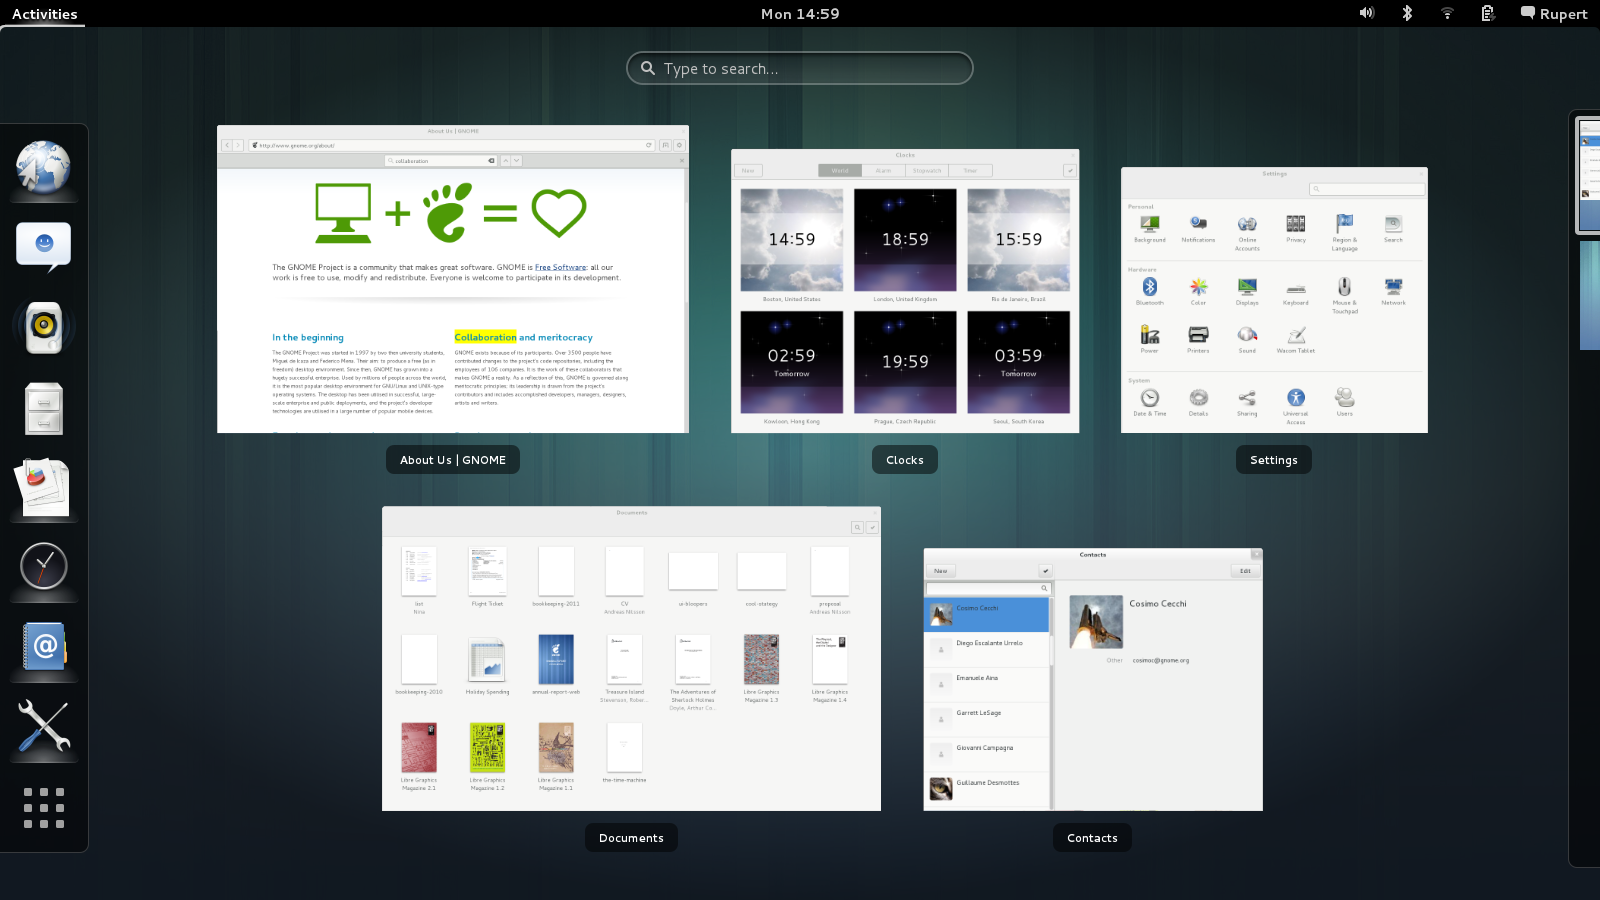
\includegraphics[width=\textwidth]{images/gui-example.png}
    \caption{Příklad GUI (zdroj: \url{https://live.gnome.org/}).}
\end{figure}

Považuji za vhodné poznamenat, že pojem \textit{grafické uživatelské rozhraní} bývá často používán výhradně pro označení rozhraní, které umožňují uživatelům komunikovat s elektronickými zařízeními (integrovaných např. v operačním systému). Tato definice je však nepřesná, neboť neoznačuje systémy, které operují jako tzv. tenký klient. Tenký klient je druh systému, jehož funkčnost je závislá na jiném zařízení (serveru). Takové systému slouží především pro projekci informací uživateli, zatímco zpracování a ukládání dat provádí server. Příkladem aplikace, která pracuje na tomto typu architektury je například Internetový prohlížeč.

\section{Webové uživatelské rozhraní}
\label{sec:wui}

Webové uživatelské rozhraní (anglicky \textit{Web-based User Interface}, dále jen WUI) je typ grafického uživatelského rozhraní, které je součástí webových aplikací. Webová aplikace je typ programu, jehož funkce a nástroje jsou přístupné přes HTTP protokol\footnote{\textit{HyperText Transfer Protocol} je internetový protokol, který definuje způsob jakým jsou data na webu formátovány a přenášeny -- původně byl tento druh komunikace zajištěn výměnou převážně hypertextových dokumentů, aktuální verze však podporuje i další formáty (XML, JSON, HTML, PDF atd.).}. Interakce mezi uživatelem a programem je pak zajištěna webovým prohlížečem.

\begin{figure}[htbp]
    \centering
    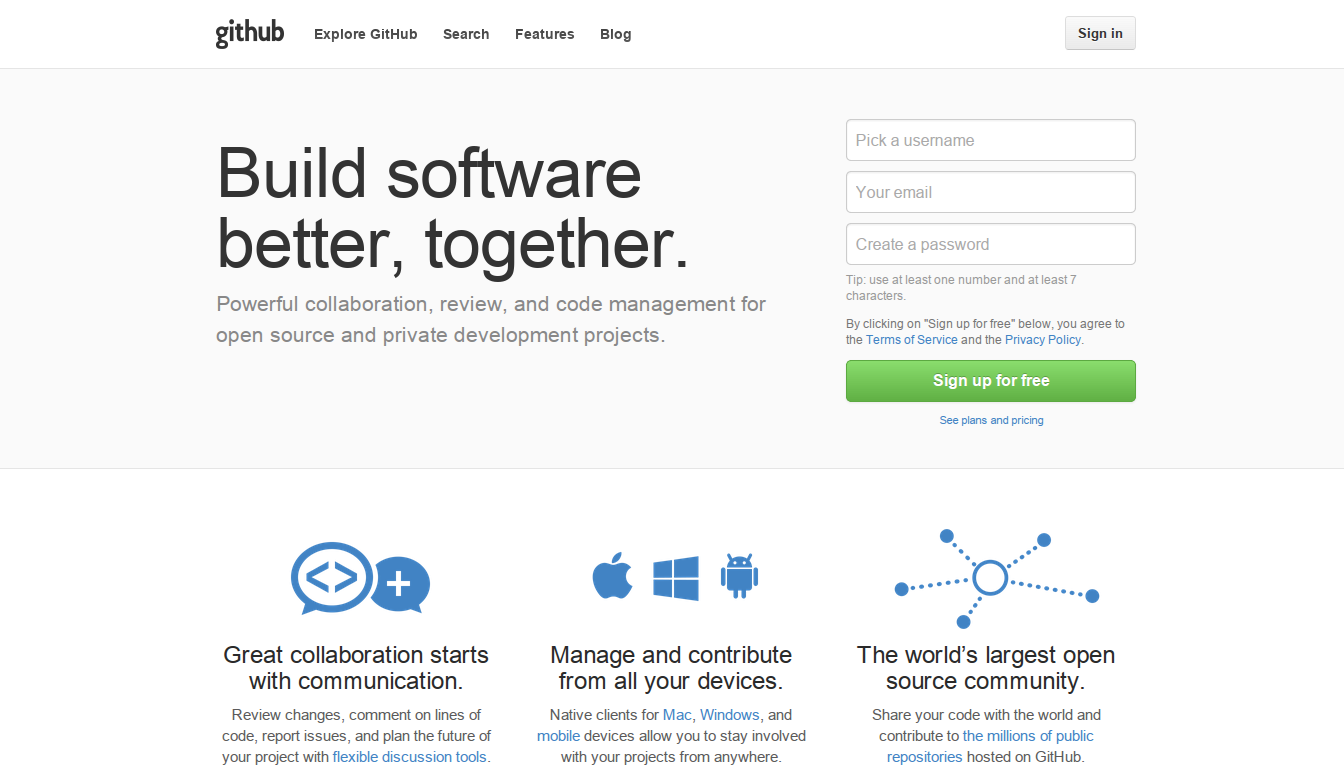
\includegraphics[width=\textwidth]{images/wui-example.png}
    \caption{Příklad WUI (zdroj: \url{https://github.com/}).}
\end{figure}

Mezi hlavní výhody webových aplikací patří relativně jednoduchá udržovatelnost a flexibilita. Tyto vlastnosti jsou dány povahou klient--server modelu. Jedná se o síťovou architekturu, která rozlišuje klienta (uživatele) a server (aplikaci). Klient--server model umožňuje vývojářům udržovat pouze jednu verzi aplikace, která je multiplatformní a často daleko bezpečnější a spolehlivější. Nevýhodou je nižší dostupnost a vyšší odezva, která je dána kvalitou síťového (Internetového) připojení.

\section{Proces tvorby uživatelského rozhraní}
\label{sec:process}

\begin{quote}
\uv{Proces tvorby uživatelského rozhraní je zdokumentovaný postup, který je nutné absolvovat pro dokončení typického uživatelského rozhraní.}
\end{quote}

\noindent
Vývoj každého systému prochází několika fázemi, které se většinou překrývají převážně z důvodu spolupráce vývojářů, designérů a analytiků. Tyto fáze lze rozdělit na čtyři části.

\begin{enumerate}[leftmargin=1cm]
    \item \textbf{Plánování}\\
          Představuje analýzu požadavků klienta a cílové skupiny uživatelů. Dále je v tomto stádiu stanoven výběr programovacích jazyků, knihoven a dalších nástrojů, které budou použity v implementaci.

    \item \textbf{Design}\\
          Informace shromážděné z předchozího stádia jsou sepsány a analyzovány. Návrh doprovází vývoj struktury a vizuální podoby aplikace, přičemž je obvykle rozdělen do tří částí -- tvorba drátěného modelu, grafického návrhu a kódování šablon. Tyto kroky mají za úkol podrobněji specifikovat požadavky klienta a odhalit nejasnosti v zadání ideálně již na počátku vývoje. Návrh probíhá převážně paralelně s vývojem.

    \item \textbf{Vývoj}\\
          V této fázi jsou požadované funkce systému implementovány za použití ustanovených technologií a knihoven. Vývoj také zahrnuje verifikaci požadavků, integraci grafických návrhů do systému a testování systému včetně použitelnosti.

    \item \textbf{Spuštění}\\
           Jedná se o poslední fázi, která prochází nejdelším cyklem. Systém je nasazen na produkci, což umožňuje hlubší testování koncovými uživateli. Zároveň jsou prováděny poslední kroky pro vypilování použitelnosti a tvorbu dokumentace.

\end{enumerate}

Produkce uživatelského rozhraní je provázána se všemi těmito fázemi a zahrnuje několik aktivit, které vyžadují práci s různými nástroji a technologiemi. Tyto aktivity vyžadují rozdílné znalosti a jsou často rozděleny mezi specificky zaměřené designéry.

\subsection{Tvorba drátěného modelu}
\label{sec:wireframing}

\begin{figure}[htbp]
    \centering
    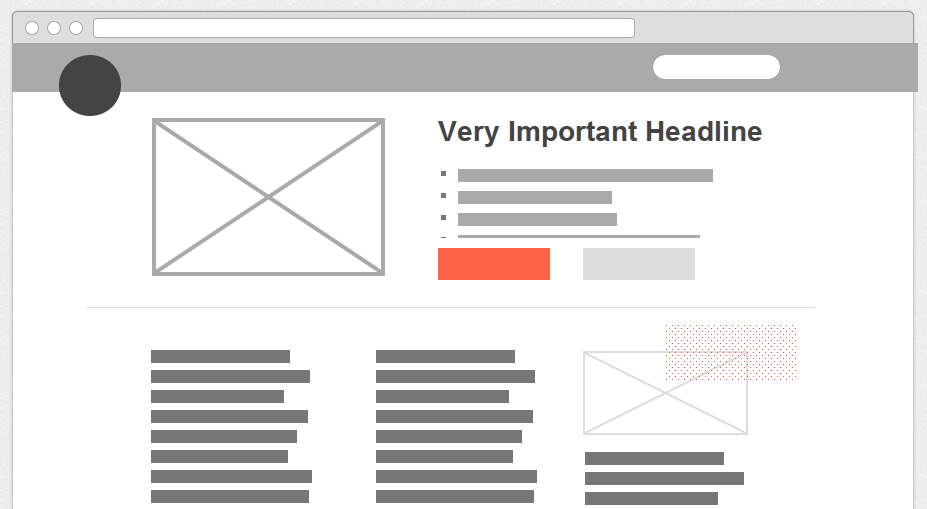
\includegraphics[width=\textwidth]{images/wireframe-example.png}
    \caption{Příklad drátěného modelu (zdroj: \url{http://wireframe.cc/}).}
\end{figure}

Webový drátěný model (anglicky \textit{wireframe}) je zjednodušená kresba, která reprezentuje rozmístění prvků a komponent webové stránky; prezentuje strukturální úroveň. Tvorba drátěného modelu zaujímá místo již na začátku životního cyklu projektu a slouží pro zachycení základní struktury stránky. Úkol drátěného modelu je poskytnout vizuální porozumění stránky již na počátku tvorby uživatelského rozhraní.

Přední výhodou drátěných modelů je jednoduchá přizpůsobitelnost potřebám klienta a jasně definovaná kostra, která zajišťuje sebedůvěru designéra. V pozdějších fázích projektu by se neměl drátěný model nijak zásadně měnit a měl by odpovídat grafickému návrhu.

\subsection{Tvorba grafického návrhu}
\label{sec:designing}

Grafický návrh poskytuje vizuální podobu webové aplikace; reprezentuje aplikaci v podobě, ve které bude prezentována uživateli. Tato fáze zahrnuje výběr grafických a typografických prvků. Mezi grafické prvky obyčejně patří kombinace barev, obrázků, tvar tlačítek apod. Typografické prvky zahrnují především organizaci písma -- volbu řezů a rodin písma pro odlišení jednotlivých částí webové stránky. Dále zahrnují velikosti odstavců, použití odrážek, řádkování atd.

\subsection{Kódování}
\label{sec:coding}

V tomto stádiu přichází na řadu rozřezání a kódování grafického návrhu. Kódování probíhá formou HTML (\textit{HyperText Markup Language}) a CSS (\textit{Cascading Style Sheets}), což jsou technologie určené primárně pro prezentaci dokumentů na webu. Kód by měl být psán s ohledem na W3C standard\footnote{W3C (\textit{World Wide Web Consortium}) je mezinárodní konsorcium, které se stará o vývoj webových standardů.}, zároveň je doporučeno dodržovat osvědčené postupy\footnote{Doporučené postupy při vývoji HTML dokumentů jsou vystaveny například společností Creative Technology (\url{http://isobar-idev.github.io/code-standards/})} pro zvýšení čitelnosti a podpory všech populárních prohlížečů.

\chapter{Design}
\label{chap:design}

Design by mohl být definován jako aktivita, jejíž úkol je přenést nápad, představu nebo myšlenku něčeho užitečného do zpracovatelné podoby, ať už se jedná o auto, budovu, službu nebo proces. Je to množina činností, která má za úkol pomoct lidem v orientaci a učinit jejich život jednodušší. Design je všudypřítomný, ať už se nacházíme uvnitř budovy, na autobusovém nástupišti nebo procházíme Internetové stránky---může to být model auta, interiér budovy nebo informační systém; představuje způsob jak věci vypadají, jak fungují a jak moc pozornosti přitahují nebo nepřitahují. Existují samozřejmě případy, kdy je nežádoucí, aby design přitahoval příliš mnoho pozornosti. Úkolem designera je tedy vžít se do role uživatele, do jeho chování a potřeb. Pouze designeři mohou proměnit koncept v něco žádoucího, hodnotného a komerčně úspěšného.

Ve 2. polovině 20. století se zrodil zcela nový obor anglicky nazvaný \textit{computer science}. Tento obor označujeme jako informatika. Informatika má zásadní vliv na design a to nejen na samotný proces tvorby, díky informačním technologiím vznikly zcela nové oblasti designu. Každá aplikace, služba nebo webová stránka potřebuje rozhraní, které bude sloužit jako vrstva komunikující s uživateli. Při vzniku prvních operačních systémů byla snaha vývojářů a designerů unifikovat grafické uživatelské rozhraní. Tato unifikace měla za úkol poskytnout uživatelům intuitivní prostředí a tím zredukovat nutnost porozumět všem variacím uživatelských rozhraní grafických aplikací. S rozšířením Internetu se toto úsilí přenáší především na designera a společnost je tak vystavena daleko většímu množství nových grafických rozhraní a technologií. Tento trend je zodpovědný za vznik mnoha nových pojmů a konvencí.

Mezi designery se v posledních letech rozšířilo několik nových termínů, které mají za úkol jednoznačně rozlišit jednotlivé činnosti a profily webdesignu. Podstatou těchto pojmů je zároveň usnadnění komunikace mezi designery, mezi ty nejpodstatnější patří---

\begin{itemize}
    \item Použitelnost (Usability)
    \item UI (User Interface)
    \item UX (User eXperience)
\end{itemize}

Tyto pojmy se navzájem prolínají. Jedná se především o soubor zásad a doporučení pro úspěšné dokončení tvorby uživatelského rozhraní.

\section{Použitelnost}
\label{sec:usability}

Použitelnost je soulad užitečnosti a jednoduchosti použití. Produkt (aplikace nebo zařízení) je použitelný pokud---

\begin{itemize}
    \item je pro uživatele užitečný a vyhovuje jeho potřebám
    \item je jednoduché naučit se produkt používat
    \item je efektivní produkt používat---zabere málo času vykonat nějaký úkol
    \item je produkt málo náchylný na chyby
\end{itemize}

Dobře použitelný produkt musí do jisté míry splňovat všechny tyto body. Existuje mnoho produktů, které jsou natolik složité, že většinu uživatelů odradí od normálního používání (pokud mají možnost volby). Často se přitom jedná o vysoce užitečné a produktivní aplikace---typickým příkladem jsou informační systémy, které obsahují ohromné množství dat a nástrojů se kterými musí uživatelé manipulovat.

\begin{figure}[htbp]
    \centering
    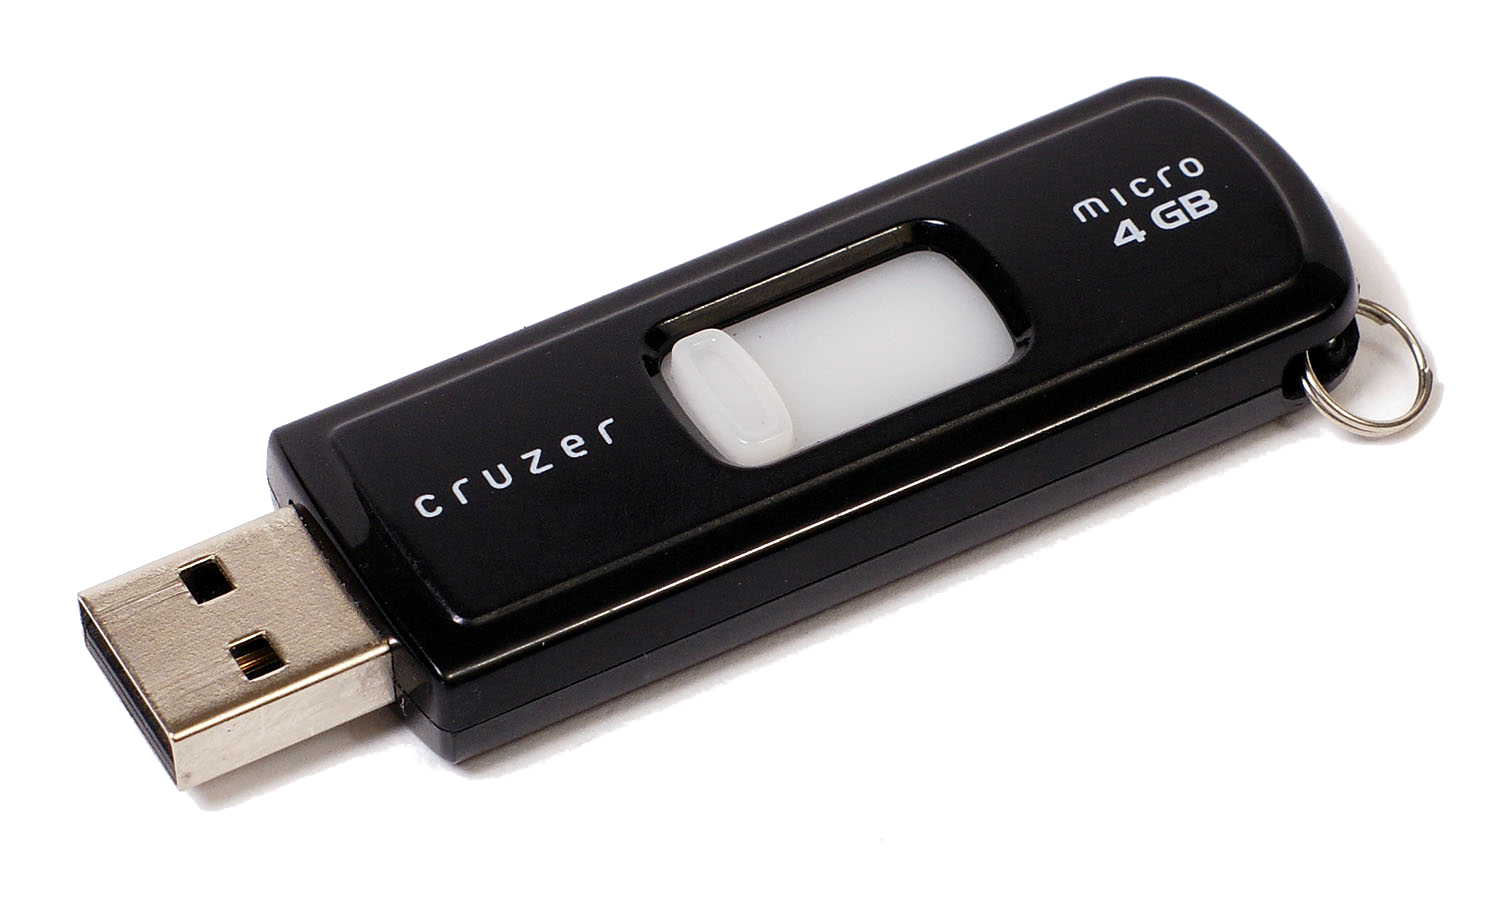
\includegraphics[width=11cm]{images/usb-fail.png}
    \caption{Špatná použitelnost USB standardu---kterou stranou se připojuje zařízení k počítači?}
\end{figure}

Mezi některé typické příklady špatné použitelnosti webových aplikací patří například absence vyhledávače, nutnost registrace pro zobrazení většiny obsahu nebo dlouhé registrační formuláře a nečitelná CAPTCHA. Jednou z nejdůležitějších vlastností dobře použitelných aplikací je správná typografie (viz \ref{sec:typografie}).

\section{UI design}
\label{sec:uidesign}

UI design zahrnuje práci designerů, kteří vytvářejí hmatatelné prvky se kterými uživatele manipulují. UI designeři se soustředí na vizuální podobu a použitelnost produktů a služeb. Použitelnost je tedy nutnou součástí kvalitních uživatelských rozhraní.

Uživatelské rozhraní webových aplikací prošlo v posledních letech zásadním vývojem---za tento vývoj je zodpovědná především rozšířenost webových technologií (HTML, CSS a JavaScript) a s tím související popularita majoritních webových prohlížečů. Ještě nedávno patřil mezi nejpopulárnější prohlížeče Internet Explorer, který má dodnes nejhorší podporu moderních webových technologií.

\section{UX design}
\label{sec:uxdesign}

UI design je část produktu, se kterou přichází uživatel do kontaktu, když se na produkt podívá. UX design je pocit, jaký uživatel má, když produkt používá \cite{ui-vs-ux}. UI design je pouze částí UX designu, stejně jako použitelnost je součástí UI designu (viz obrázek \ref{fig:ux-ui-usability}).

\begin{figure}[htbp]
    \centering
    \includegraphics[width=10cm]{images/ux.pdf}
    \caption{Podíl UX, UI a použitelnosti v designu.}
    \label{fig:ux-ui-usability}
\end{figure}

Příklad některých prvků, které mají vliv na dobrý UX design \cite{understanding-ux-ui}.

\begin{itemize}
    \item \textbf{Obsah}. Kvalita obsahu, struktura textu obrázků a dalších typografických prvků.
    \item \textbf{Dostupnost pomoci}. Online chat, email technické podpory.
    \item \textbf{Výkon}. Rychlost stránek a dostupnost.
    \item \textbf{Diskuze}. Podpora diskuzí a hodnocení produktů.
    \item \textbf{Způsob platby}. Možnost internetové platby (platba kartou, PayPal apod.)
    \item \textbf{Reklama}. Výskyt reklam a jejich způsob zobrazení.
\end{itemize}

\section{Typografie}
\label{sec:typografie}

\begin{quote}
    \uv{Typografie je organizace písma v ploše} \cite{svalbach}
\end{quote}

\noindent
Typografie je ještě starší než samotný design, její počátky sahají do 15. století, kdy Johannes Gutenberg vynalezl knihtisk. Už tehdy si typografové uvědomovali její důležitost. Během nadcházejících století se typografie rozšířila do novin, informačních systémů nebo reklam. Popularita typografie měla za následek rozvoj mnoha rodin písma, které se používají i u dnešních displejů elektronických zařízení.

Webdesign je z 95\% typografie---toto tvrzení vyplývá ze skutečnosti, že 95\% informací na internetu se nachází v písemné podobě \cite{typography}. Typografie je zásadním prvkem pro tvorbu webových aplikací, jedná se o primární způsob přenosu informací mezi aplikací a uživatelem. Tento fakt klade určité nároky na kvalitní uživatelská rozhraní, které vycházejí z knižní typografie.

\subsection{Volba čitelných fontů}

Pro nadpisy a podnadpisy je doporučené používat patkové písmo, naopak pro menší text bezpatkové. Displeje s nízkým PPI (počtem pixelů na palec) radikálně snižují čitelnost patkových fontů.

\subsection{Šířka odstavců}

Příliš dlouhé řádky textu snižují soustředěnost. Tento jev je dán nutností čtenáře získat představu o tom, kde řádek končí a kde nový začíná. Naopak krátké řádky nutí návštěvníka číst příliš přerušovaně. Délka odstavce by měla odpovídat přibližně 55--80 znakům na řádek.

\subsection{Velikost písma}

Minimální doporučovaná velikost písma je 16$px$, což je přibližně stejná velikost, jako velikost textu vytištěného v knize nebo v magazínu \cite{min-font-size}.

\subsection{Řádkování}

Podobně jako šířka odstavců i řádkování ovlivňuje nutnost koncentrace čtenáře. Minimální doporučené řádkování je 1.3$em$.

\subsection{Velikost okrajů}

Okraje oddělují důležitý obsahu od ostatních částí webu a dovolují čtenáři soustředit se na text. Doporučený poměr okrajů na webu je 2:3:4:3 (vrch \textbf{:} pravá strana \textbf{:} spodek \textbf{:} levá strana), velikost okrajů pak 2$em$ \textbf{:} 3$em$ \textbf{:} 4$em$ \textbf{:} 3$em$, kde 1$em$ je roven dvojnásobku velikosti fontu.

\subsection{Kontrast textu}

Kontrast má velký vliv na čitelnost, nízký kontrast zvyšuje únavu očí, naopak příliš vysoký kontrast působí dráždivě \cite{eye-strain}. Jedna z doporučených kombinací je tmavě šedý text na bílém pozadí.

\begin{figure}[htbp]
    \centering
    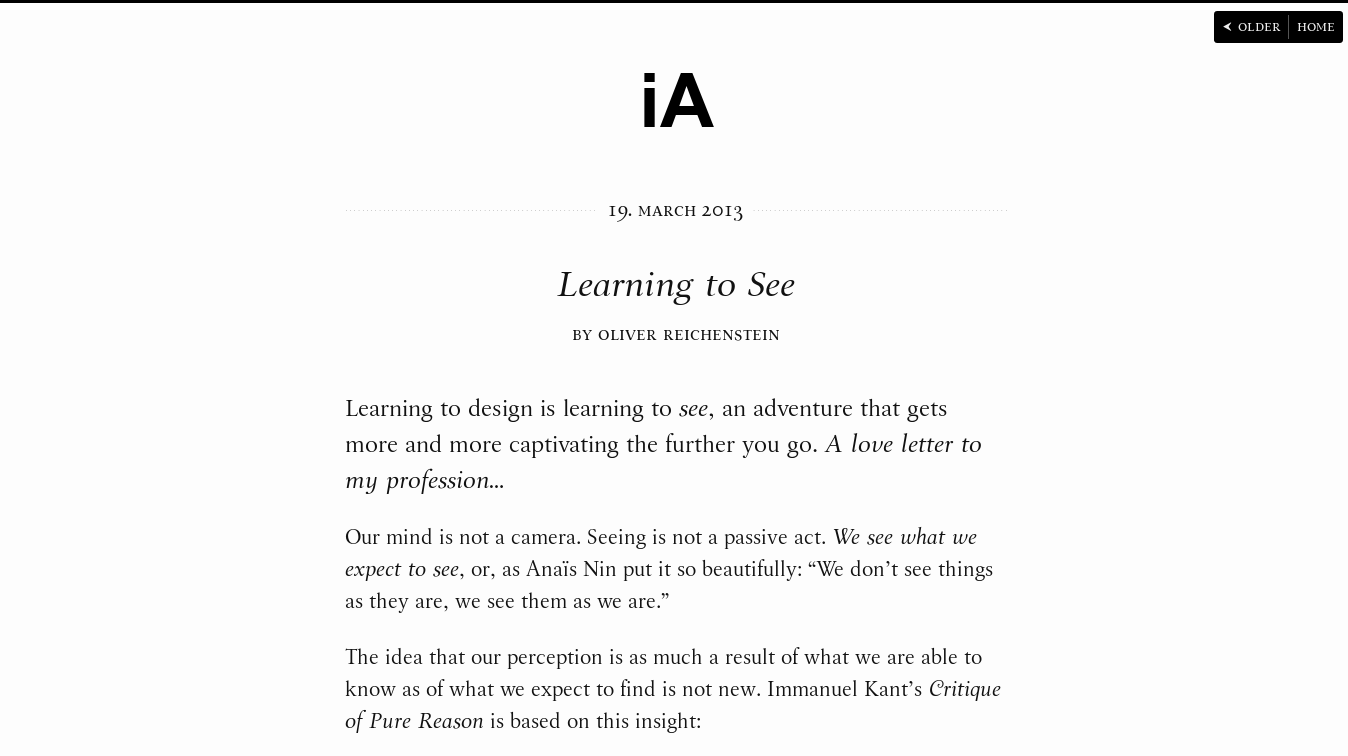
\includegraphics[width=11cm]{images/typography.png}
    \caption{Příklad webové stránky, kde autor použil výhradně typografické prvky. Na stránce si můžeme všimnout použití pouze jedné rodiny písma. Zdroj: \url{http://informationarchitects.net/}.}
    \label{fig:web-typography}
\end{figure}

\chapter{Design}
\label{chap:design}

Design by mohl být definován jako aktivita, jejíž úkol je přenést nápad, představu nebo myšlenku něčeho užitečného do zpracovatelné podoby, ať už se jedná o auto, budovu, službu nebo proces. Je to množina činností, která má za úkol pomoct lidem v orientaci a učinit jejich život jednodušší. Design je všudypřítomný, ať už se nacházíme uvnitř budovy, na autobusovém nástupišti nebo procházíme Internetové stránky---může to být model auta, interiér budovy nebo informační systém; představuje způsob jak věci vypadají, jak fungují a jak moc pozornosti přitahují nebo nepřitahují. Existují samozřejmě případy, kdy je nežádoucí, aby design přitahoval příliš mnoho pozornosti. Úkolem designera je tedy vžít se do role uživatele, do jeho chování a potřeb. Pouze designeři mohou proměnit koncept v něco žádoucího, hodnotného a komerčně úspěšného.

Ve 2. polovině 20. století se zrodil zcela nový obor anglicky nazvaný \textit{computer science}. Tento obor označujeme jako informatika. Informatika má zásadní vliv na design a to nejen na samotný proces tvorby, díky informačním technologiím vznikly zcela nové oblasti designu. Každá aplikace, služba nebo webová stránka potřebuje rozhraní, které bude sloužit jako vrstva komunikující s uživateli. Při vzniku prvních operačních systémů byla snaha vývojářů a designerů unifikovat grafické uživatelské rozhraní. Tato unifikace měla za úkol poskytnout uživatelům intuitivní prostředí a tím zredukovat nutnost porozumět všem variacím uživatelských rozhraní grafických aplikací. S rozšířením Internetu se toto úsilí přenáší především na designera a společnost je tak vystavena daleko většímu množství nových grafických rozhraní a technologií. Tento trend je zodpovědný za vznik mnoha nových pojmů a konvencí.

Mezi designery se v posledních letech rozšířilo několik nových termínů, které mají za úkol jednoznačně rozlišit jednotlivé činnosti a profily webdesignu. Podstatou těchto pojmů je zároveň usnadnění komunikace mezi designery, mezi ty nejpodstatnější patří---

\begin{itemize}
    \item Použitelnost (Usability)
    \item UI (User Interface)
    \item UX (User eXperience)
\end{itemize}

Tyto pojmy se navzájem prolínají. Jedná se především o soubor zásad a doporučení pro úspěšné dokončení tvorby uživatelského rozhraní.

\section{Použitelnost}
\label{sec:usability}

Použitelnost je soulad užitečnosti a jednoduchosti použití. Produkt (aplikace nebo zařízení) je použitelný pokud---

\begin{itemize}
    \item je pro uživatele užitečný a vyhovuje jeho potřebám
    \item je jednoduché naučit se produkt používat
    \item je efektivní produkt používat---zabere málo času vykonat nějaký úkol
    \item je produkt málo náchylný na chyby
\end{itemize}

Dobře použitelný produkt musí do jisté míry splňovat všechny tyto body. Existuje mnoho produktů, které jsou natolik složité, že většinu uživatelů odradí od normálního používání (pokud mají možnost volby). Často se přitom jedná o vysoce užitečné a produktivní aplikace---typickým příkladem jsou informační systémy, které obsahují ohromné množství dat a nástrojů se kterými musí uživatelé manipulovat.

\begin{figure}[htbp]
    \centering
    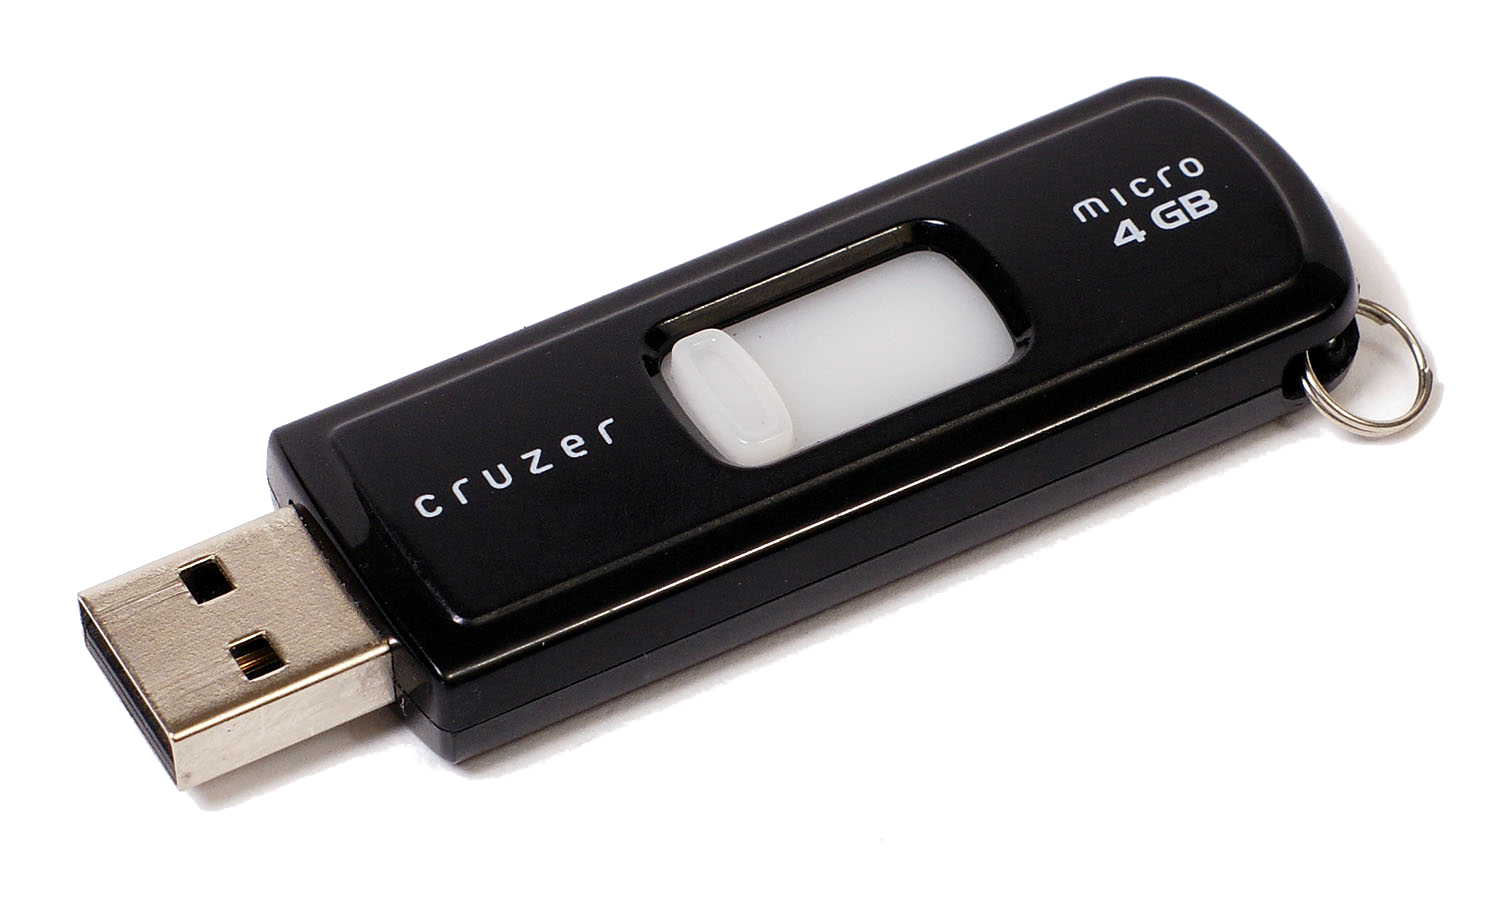
\includegraphics[width=11cm]{images/usb-fail.png}
    \caption{Špatná použitelnost USB standardu---kterou stranou se připojuje zařízení k počítači?}
\end{figure}

Mezi některé typické příklady špatné použitelnosti webových aplikací patří například absence vyhledávače, nutnost registrace pro zobrazení většiny obsahu nebo dlouhé registrační formuláře a nečitelná CAPTCHA. Jednou z nejdůležitějších vlastností dobře použitelných aplikací je správná typografie (viz \ref{sec:typografie}).

\section{UI design}
\label{sec:uidesign}

UI design zahrnuje práci designerů, kteří vytvářejí hmatatelné prvky se kterými uživatele manipulují. UI designeři se soustředí na vizuální podobu a použitelnost produktů a služeb. Použitelnost je tedy nutnou součástí kvalitních uživatelských rozhraní.

Uživatelské rozhraní webových aplikací prošlo v posledních letech zásadním vývojem---za tento vývoj je zodpovědná především rozšířenost webových technologií (HTML, CSS a JavaScript) a s tím související popularita majoritních webových prohlížečů. Ještě nedávno patřil mezi nejpopulárnější prohlížeče Internet Explorer, který má dodnes nejhorší podporu moderních webových technologií.

\section{UX design}
\label{sec:uxdesign}

UI design je část produktu, se kterou přichází uživatel do kontaktu, když se na produkt podívá. UX design je pocit, jaký uživatel má, když produkt používá \cite{ui-vs-ux}. UI design je pouze částí UX designu, stejně jako použitelnost je součástí UI designu (viz obrázek \ref{fig:ux-ui-usability}).

\begin{figure}[htbp]
    \centering
    \includegraphics[width=10cm]{images/ux.pdf}
    \caption{Podíl UX, UI a použitelnosti v designu.}
    \label{fig:ux-ui-usability}
\end{figure}

Příklad některých prvků, které mají vliv na dobrý UX design \cite{understanding-ux-ui}.

\begin{itemize}
    \item \textbf{Obsah}. Kvalita obsahu, struktura textu obrázků a dalších typografických prvků.
    \item \textbf{Dostupnost pomoci}. Online chat, email technické podpory.
    \item \textbf{Výkon}. Rychlost stránek a dostupnost.
    \item \textbf{Diskuze}. Podpora diskuzí a hodnocení produktů.
    \item \textbf{Způsob platby}. Možnost internetové platby (platba kartou, PayPal apod.)
    \item \textbf{Reklama}. Výskyt reklam a jejich způsob zobrazení.
\end{itemize}

\section{Typografie}
\label{sec:typografie}

\begin{quote}
    \uv{Typografie je organizace písma v ploše} \cite{svalbach}
\end{quote}

\noindent
Typografie je ještě starší než samotný design, její počátky sahají do 15. století, kdy Johannes Gutenberg vynalezl knihtisk. Už tehdy si typografové uvědomovali její důležitost. Během nadcházejících století se typografie rozšířila do novin, informačních systémů nebo reklam. Popularita typografie měla za následek rozvoj mnoha rodin písma, které se používají i u dnešních displejů elektronických zařízení.

Webdesign je z 95\% typografie---toto tvrzení vyplývá ze skutečnosti, že 95\% informací na internetu se nachází v písemné podobě \cite{typography}. Typografie je zásadním prvkem pro tvorbu webových aplikací, jedná se o primární způsob přenosu informací mezi aplikací a uživatelem. Tento fakt klade určité nároky na kvalitní uživatelská rozhraní, které vycházejí z knižní typografie.

\subsection{Volba čitelných fontů}

Pro nadpisy a podnadpisy je doporučené používat patkové písmo, naopak pro menší text bezpatkové. Displeje s nízkým PPI (počtem pixelů na palec) radikálně snižují čitelnost patkových fontů.

\subsection{Šířka odstavců}

Příliš dlouhé řádky textu snižují soustředěnost. Tento jev je dán nutností čtenáře získat představu o tom, kde řádek končí a kde nový začíná. Naopak krátké řádky nutí návštěvníka číst příliš přerušovaně. Délka odstavce by měla odpovídat přibližně 55--80 znakům na řádek.

\subsection{Velikost písma}

Minimální doporučovaná velikost písma je 16$px$, což je přibližně stejná velikost, jako velikost textu vytištěného v knize nebo v magazínu \cite{min-font-size}.

\subsection{Řádkování}

Podobně jako šířka odstavců i řádkování ovlivňuje nutnost koncentrace čtenáře. Minimální doporučené řádkování je 1.3$em$.

\subsection{Velikost okrajů}

Okraje oddělují důležitý obsahu od ostatních částí webu a dovolují čtenáři soustředit se na text. Doporučený poměr okrajů na webu je 2:3:4:3 (vrch \textbf{:} pravá strana \textbf{:} spodek \textbf{:} levá strana), velikost okrajů pak 2$em$ \textbf{:} 3$em$ \textbf{:} 4$em$ \textbf{:} 3$em$, kde 1$em$ je roven dvojnásobku velikosti fontu.

\subsection{Kontrast textu}

Kontrast má velký vliv na čitelnost, nízký kontrast zvyšuje únavu očí, naopak příliš vysoký kontrast působí dráždivě \cite{eye-strain}. Jedna z doporučených kombinací je tmavě šedý text na bílém pozadí.

\begin{figure}[htbp]
    \centering
    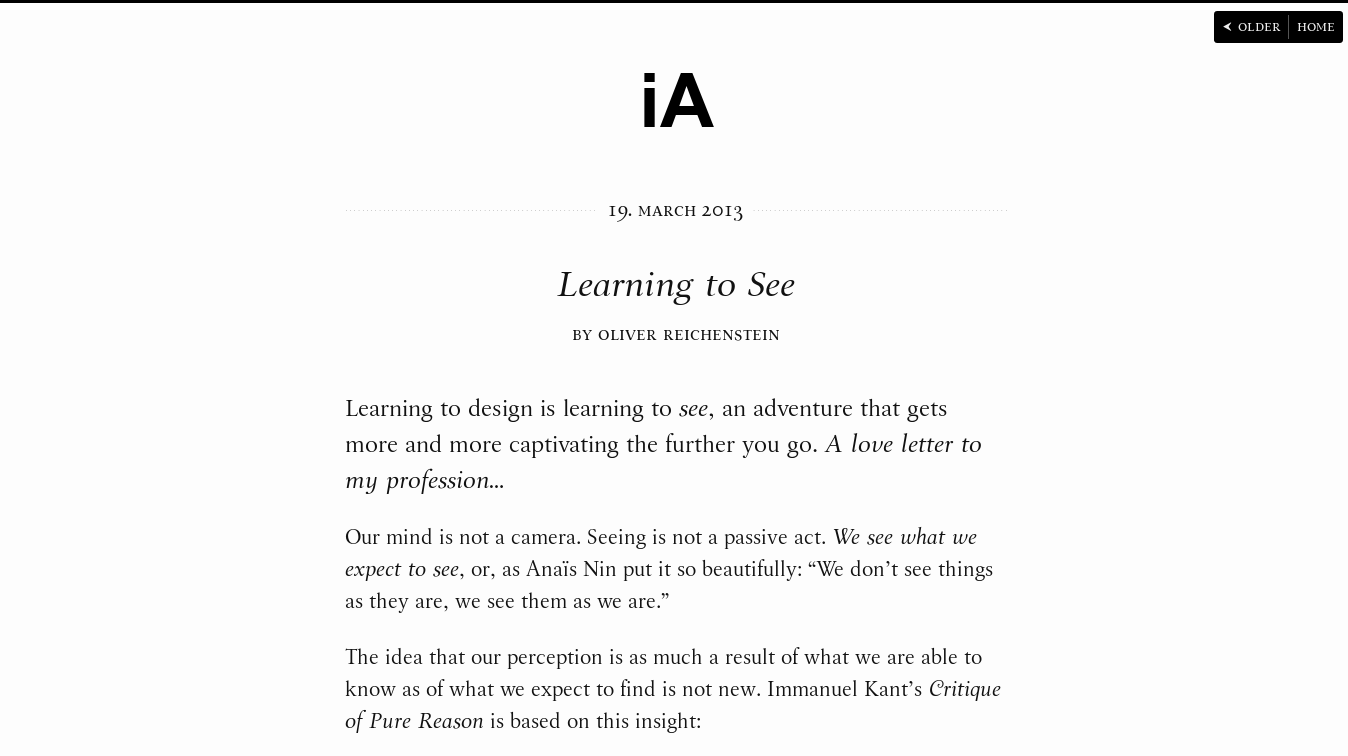
\includegraphics[width=11cm]{images/typography.png}
    \caption{Příklad webové stránky, kde autor použil výhradně typografické prvky. Na stránce si můžeme všimnout použití pouze jedné rodiny písma. Zdroj: \url{http://informationarchitects.net/}.}
    \label{fig:web-typography}
\end{figure}

\chapter{Značkovací a stylovací jazyky}
\label{chap:languages}

\section{HTML}
\label{sec:html}

\section{CSS}
\label{sec:css}

\section{LESS}
\label{sec:less}

\section{Twitter Bootstrap}
\label{sec:bootsrap}




\cite{groovy-in-action}

\bibliographystyle{IEEEtran}
\bibliography{index}

\end{document}
